% Part: normal-modal-logic
% Chapter: filtrations
% Section: more-filtrations

\documentclass[../../../include/open-logic-section]{subfiles}

\begin{document}

\olfileid{mod}{fil}{acc}

\olsection{Filtrations and Properties of Accessibility}

\begin{defn}
  Let $\Gamma$ be closed under subformulas and $\mModel{M} =\tuple{W, R, V}$ a
  model. Then we can define conditions on pairs of worlds $u,v$ as given in
  the table of \olref{fig:Cn-filtrations}. 
\end{defn}

  \begin{figure}[ht]
    \centering
    \begin{tabular}{|ll|}
      \hline
      \multirow{2}{*}{$C_1(u,v)$:}  &if $\Box!A \in \Gamma$  and $\mSat{M}{\Box!A}[u]$ then $\mSat{M}{!A}[v]$; and \\
      & if $\Diamond!A \in \Gamma$  and $\mSat{M}{!A}[v]$ then $\mSat{M}{\Diamond!A}[u]$; \\
      \hline
      \multirow{2}{*}{$C_2(u,v)$:} &if $\Box!A \in \Gamma$  and $\mSat{M}{\Box!A}[v]$ then $\mSat{M}{!A}[u]$; and \\
      & if $\Diamond!A \in \Gamma$  and $\mSat{M}{!A}[u]$ then $\mSat{M}{\Diamond!A}[v]$; \\
      \hline
      \multirow{2}{*}{$C_3(u,v)$:} &if $\Box!A \in \Gamma$  and $\mSat{M}{\Box!A}[u]$ then $\mSat{M}{\Box!A}[v]$; and \\
      & if $\Diamond!A \in \Gamma$  and $\mSat{M}{\Diamond!A}[v]$ then $\mSat{M}{\Diamond!A}[u]$; \\
      \hline
      \multirow{2}{*}{$C_4(u,v)$:} &if $\Box!A \in \Gamma$  and $\mSat{M}{\Box!A}[v]$ then $\mSat{M}{\Box!A}[u]$; and \\
      & if $\Diamond!A \in \Gamma$  and $\mSat{M}{\Diamond!A}[u]$ then $\mSat{M}{\Diamond!A}[v]$; \\
      \hline
    \end{tabular}
    \caption{Conditions on possible worlds for defining
      filtrations.}\ollabel{fig:Cn-filtrations}
\end{figure}

\begin{thm}\ollabel{thm:more-filtrations}
  Let $\mModel{M} =\tuple{W,R,P}$ be a model, $\Gamma$ closed under
  subformulas. Let $W^*$ and $V^*$ be defined as in
  \olref[fil]{def:filtration}. Then:
  \begin{enumerate}
  \item If $R^*$ is defined as $R^*[u][v]$ if and only if $C_1(uv)
    \land C_2(u,v)$ then $R^*$ is symmetric, and
    $\mModel{M^*} = \tuple{W^*,R^*,V^*}$ is a filtration if $\mModel{M}$
    is symmetric.
  \item If $R^*$ is defined as $R^*[u][v]$ if and only if $C_1(uv)
    \land C_3(u,v)$ then $R^*$ is transitive, and
    $\mModel{M^*}=\tuple{W^*,R^*,V^*}$ is a filtration if $\mModel{M}$
    is transitive.
  \item If $R^*$ is defined as $R^*[u][v]$ if and only if $C_1(uv)
    \land C_2(u,v) \land C_3(u,v) \land C_4(u,v)$ then $R^*$ is
    symmetric and transitive, and $\mModel{M^*}=\tuple{W^*,R^*,V^*}$
    is a filtration if $\mModel{M}$ is symmetric and transitive.
  \item If $R^*$ is defined as $R^*[u][v]$ if and only if $C_1(uv)
    \land C_3(u,v) \land C_4(u,v)$ then $R^*$ is transitive and
    euclidean, and $\mModel{M^*}=\tuple{W^*,R^*,V^*}$ is a filtration
    if $\mModel{M}$ is transitive and euclidean.
  \end{enumerate}
\end{thm}

\begin{proof}
  \begin{enumerate}
    \item It's immediate that $R^*$ is symmetric, since $C_1(u,v)
      \Leftrightarrow C_2(v,u)$ and $C_2(u,v) \Leftrightarrow
      C_1(v,u)$. So it's left to show that if $\mModel{M}$ is
      symmetric then $\mModel{M^*}$ is a filtration through
      $\Gamma$. By condition $C_1(u,v)$ we get that: if $\Box!A \in
      \Gamma$ and $\mSat{M}{\Box!A}[u]$ then $\mSat{M}{!A}[v]$, and if
      $\Diamond!A \in \Gamma$ and $\mSat{M}{!A}[v]$ then
      $\mSat{M}{\Diamond!A}[u]$. So all we need is that $Ruv$ implies
      $R^*[u][v]$.

      So suppose $Ruv$, to show $R^*[u][v]$ we need $C_1(u,v) \land
      C_2(u,v)$. For $C_1$: if $\Box!A \in\Gamma$ and
      $\mSat{M}{\Box!A}[u]$ then also $\mSat{M}{!A}[v]$ (since $Ruv$);
      and similarly if $\Diamond!A \in \Gamma$ and $\mSat{M}{!A}[v]$
      then $\mSat{M}{\Diamond!A}[u]$. For $C_2$: if $\Box!A \in
      \Gamma$ and $\mSat{M}{\Box!A}[v]$ then $Ruv$ implies $Rvu$ by
      symmetry, so that $\mSat{M}{!A}[u]$; similarly if $\Diamond!A
      \in\Gamma$ and $\mSat{M}{!A}[u]$ then $\mSat{M}{\Diamond!A}[v]$
      (since $Rvu$ by symmetry).
    \item Exercise.
    \item Exercise.
    \item Exercise.
  \end{enumerate}
\end{proof}

\begin{prob}
  Complete the proof of \olref[mod][fil]{thm:more-filtrations}.
\end{prob}

This approach does not work in the case of models that are euclidean
or serial and euclidean. Consider the model at the top of
Figure~\olref{fig:ser-eucl}, which is both euclidean and serial. Let
$\Gamma = \{p, \Box p \}$. When taking a filtration through $\Gamma$,
then $[w_1] = [w_3]$ since $w_1$ and $w_3$ are the only worlds that
agree on $\Gamma$. Any filtration will also have the arrow inherited
from $\mModel{M}$, as depicted in Figure~\olref{fig:ser-eucl2}. But we
cannot add arrows to that model in order to make it euclidean, for
then there would be a double arrow between $w_2$ and $w_4$, and hence
also between $w_2$ and $w_5$. But $\Box p$ is true at $w_2$ while $p$
is false at $w_5$.

\begin{figure}[htpb]
  \centering
  \begin{tikzpicture}[node distance=2cm, auto, thick]
    \node (w1) at (0, 0) [label=90:$w_1$, label=below:$\lnot p$]{$\bullet$}; 
    \node (w2) at (2, 0) [label=90:$w_2$, label=below:$p$]{$\bullet$}; 
    \draw[->] (w1) to node {} (w2);
    \path node at (0,-1) {$\Box p$};
    \path node at (2,-1) {$\Box p$};
    \node (w3) at (0, -2.5) [label=90:$w_3$, label=below:$\lnot p$]{$\bullet$}; 
    \node (w4) at (2, -2.5) [label=135:$w_4$,
      label=below:$p$]{$\bullet$}edge [in=60,out=120,loop] (); 
    \draw[->] (w3) to node {} (w4);
    \node (w5) at (4, -2.5) [label=90:$w_5$, label=below:$\lnot p$]{$\bullet$}; 
    \draw[<->] (w4) to node {} (w5) edge [in=30,out=-30,loop] () ;
    \path node at (0,-3.5) {$\Box p$};
    \path node at (2,-3.5) {$\lnot\Box p$};
    \path node at (4,-3.5) {$\lnot\Box p$};
    \draw [rounded corners] (-1,-4) -- ++(6.25,0)  -- ++(0,5) -- ++(-6.25,0) --  cycle;
    % \draw[->, bend left] (w1) to node {$R$} (w2); 
    % \draw[->, bend left] (w2) to node {} (w1); 
    % \draw [rounded corners] (-1,-1) -- ++(0,2)  -- ++(4.25,0) -- ++(0,-2) --  cycle;
    % \path node at (2.75,0.75) {$\mModel{M}$};
  \end{tikzpicture}
  \caption{A serial and euclidean model.}\ollabel{fig:ser-eucl}
\end{figure}

\begin{figure}[ht]
  \centering
  \begin{tikzpicture}[node distance=2cm, auto, thick]
    \node (w1) at (-0.5, -1) [label=110:{$[w_1]=[w_3]$}, label=below:$\lnot
      p$]{$\bullet$}; 
    \path node at (-0.5,-2) {$\Box p$};
    \node (w2) at (2, 0) [label=90:$w_2$,
      label=0:{$p, \Box p$}]{$\bullet$}; 
    \node (w4) at (2, -2.5) [label=210:$w_4$,
      label=below:$p$]{$\bullet$}edge [in=60,out=120,loop] (); 
    \draw[->] (w1) to node {} (w2);
    \draw[->] (w1) to node {} (w4);
    \node (w5) at (4, -2.5) [label=90:$w_5$, label=below:$\lnot p$]{$\bullet$}; 
    \draw[<->] (w4) to node {} (w5) edge [in=30,out=-30,loop] () ;
    \path node at (2, -3.5) {$\lnot\Box p$};
    \path node at (4, -3.5) {$\lnot\Box p$};
    \draw [rounded corners] (-3,-4) -- ++(8.25,0)  -- ++(0,5) -- ++(-8.25,0) --  cycle;
  \end{tikzpicture}
  \caption{The filtration from the model in Figure~\olref{fig:ser-eucl}.}
  \ollabel{fig:ser-eucl2}
\end{figure}

In particular, it is not enough to consider filtrations through
arbitrary $\Gamma$'s closed under subsentences. Instead we need to
consider sets $\Gamma$ that are \emph{modally closed} (see
\olref{def:modallyclosed}). Such sets of sentences are
infinite, and therefore do not lead immediately to the decidability of
the corresponding system.

\begin{thm}
  Let $\Gamma$ be modally closed and $\mModel{M}=\tuple{W,R,V}$. If
  $\mModel{M^*} = \tuple{W^*,R^*,V^*}$ is a coarsest filtration of
  $\mModel{M}$, then $\mModel{M^*}$ is symmetric, transitive or
  euclidean if $\mModel{M}$ is symmetric, transitive, or euclidean,
  respectively.
\end{thm}

\begin{proof}
  The proof of transitivity uses the validity of both \Ax{4} and
  $\mathsf{4_\Diamond}$ in all transitive models, and likewise
  euclideanness uses the fact that both \Ax{5} and
  $\mathsf{5_\Diamond}$ are valid in all euclidean models, and the
  proof of symmetry likewise uses both \Ax{B} and
  $\mathsf{B_\Diamond}$.

  If $\mModel{M^*}$ is a coarsest filtration, then by definition
  $R^*[u][v]$ holds if and only if $C_1(u,v)$. For transitivity,
  suppose $C_1(u,v)$ and $C_1(v,w)$: to show $C_1(u,w)$ suppose
  $\mSat{M}{\Box !A}[u]$; then $\mSat{M}{\Box\Box!A}[u]$; since
  $\Box\Box!A \in \Gamma$ by closure, also by $C_1(u,v)$,
  $\mSat{M}{\Box!A}[v]$ and by $C_1(v,w)$, also $\mSat{M}{!A}[w]$. The
  case for $\Diamond!A$ is similar.
\end{proof}

\part{Problem sets}

\section{Problem set 1: understanding Kripke semantics}


\begin{problem} [60 points]
  Consider the following model ${M}$ for the language
  comprising $p_1, p_2, p_3$ as the only propositional variables:
%% See: http://pdp7.org/blog/?p=133
\begin{center}
  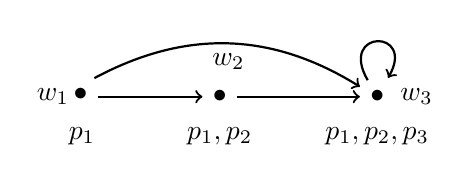
\begin{tikzpicture}[node distance=2cm, auto, thick]
    \node (w1) {$w_1 \, \bullet$} ; 
    \node (w2) [right of=w1]
    {$\bullet$}; 
    \node (w3) [right of=w2] {$\bullet$} edge
    [in=60,out=120,loop] () ;
    \draw[->] (w1) to node {} (w2); \draw[->] (w2) to node {} (w3);
    \draw[->, bend left] (w1) to node [swap] {$w_2$} (w3); 
    \path node at ( 4.5,0) {$w_3$}; 
    \path node at ( 0.25,-0.5) {$p_1$}; 
    \path node at ( 2,-0.5) {$p_1,p_2$}; 
    \path node at ( 4,-0.5) {$p_1,p_2,p_3$};
    % \path node at ( 0,-1) [shape=circle,draw] {};
  \end{tikzpicture}
%\node [circle,draw] {a} edge [in=30,out=60,loop] ();
\end{center}
Are the following !!{formula}s and schemas true in the model ${M}$,
i.e., true at every world in ${M}$? Explain.
\begin{enumerate}
\item $p\lif \Diamond p$ (for $p$ atomic);
\item $!A\lif \Diamond !A$ (for $!A$ arbitrary);
\item $\Box p \lif p$ (for $p$ atomic);
\item $\lnot p \lif \Diamond \Box p$ (for $p$ atomic);
\item $\Diamond \Box !A$ (for $!A$ arbitrary);
\item $\Box \Diamond p$ (for $p$ atomic). 
\end{enumerate}
\end{problem}


\begin{problem} [20 points]
For each of the following !!{formula}s find a model ${M} = \tuple{W, R V}$ and a
world $w \in W$ such that the !!{formula} fails at $w$:
\begin{enumerate}
\item $p \lif \Box\Box p$;
\item $\Box(p \lor q) \lif (\Box p \lor \Box q)$.
\end{enumerate}
\end{problem}

\begin{problem} [20 points]
For each of the following schemas find a model $\mathbf{M}$ such that
every instance of the schema is true in $\mathbf{M}$:
\begin{enumerate}
\item $!A \lif \Diamond\Diamond !A$;
\item $\Diamond !A \lif \Box !A$.
\end{enumerate}
\end{problem}


\section{Problem set 2: provability}
\setcounter{problem}{0}

\begin{definition}
  Given a normal system $\Sigma$ of modal logic, say that $!A$ is
  \emph{!!{derivable}} in $\Sigma$, written $\Sigma \Proves !A$, if and
  only if there is a proof of $!A$ from axioms in $\Sigma$ using
  \MP{} and \Nec{}. Equivalently, $!A$ belongs to the smallest set of
  sentences containing $\Sigma$ and closed under tautological
  implication and \RK{}.
\end{definition}

\begin{problem} [24 points]
  Provide $\Log{K}$-proofs of the following:
\begin{enumerate}
\item $\Diamond \lnot \lfalse \lif (\Box !A \lif \Diamond !A)$;
\item $\Box(!A \lor !B) \lif (\Diamond !A \lor \Box !B)$;
\item $(\Diamond !A \lif \Box !B) \lif \Box(!A \lif !B)$.
\end{enumerate}
\end{problem}

For ease of reference, we restate here \olref{thm:soundness}:

\noindent
\textbf{Soundness Theorem}: if schemas
$!A_1, \dots,!A_n$ are valid in the classes of models
$\mClass{C}_n, \dots,\mClass{C}_n$, respectively, then
$\Log{K}!A_1\dots !A_n \Proves !B$ implies
that $!B$ is valid in the class of models $\mClass{C}_n \cap
\dots \cap \mClass{C}_n$.


\begin{definition}
  An inference rule of the form 
\[
{!A_1 \dots !A_n} \over !B \eqno{(*)\hspace{2in}}
\]
is \emph{admissible} in a system $\Sigma$ if and only if, whenever
$\Sigma \Proves !A_i$ for $i =1, \dots,n$, then also $\Sigma
\Proves !B$. In other words, adding the new rule to the system does
not change the set of !!{derivable} !!{formula}s.
\end{definition}

\begin{definition}
  An inference rule of the form $(*)$ is \emph{derivable} in a system
  $\Sigma$ if and only if $\Sigma \Proves !A_1 \lif (!A_2 \to
  ( \cdots (!A_n \lif !B) \cdots)$.
\end{definition}

\begin{problem} [6 points]
  Show that if a rule is derivable in $\Sigma$ then it is admissible
  in $\Sigma$. 
\end{problem}

\begin{definition}
  Define a function $\sigma$ from !!{formula}s into !!{formula}s recursively
  by setting:
  \begin{eqnarray*}
    \sigma(p) & = & p ;\\
   \sigma(\lfalse) & = &  \lfalse ;\\
    \sigma(\lnot !A) & = & \lnot\sigma(!A);\\
   \sigma(!A \lif !B) & = & \sigma(!A) \lif \sigma(!B);\\
   \sigma(\Box !A) & = & !A.
  \end{eqnarray*}
  So $\sigma$ erases the outermost occurrence of $\Box$.  For
  instance, compute $\sigma(\Box(\Diamond A \lif \Diamond\Box B))$ and
  $\sigma(\Diamond A \lif \Diamond\Box B)$
% (after re-writing $\Diamond$ as $\lnot\Box\lnot$)
.
\end{definition}

\goodbreak



\begin{problem} [20 points]
  Show that if $\Log{K}\Proves !A$ then $\Log{K}\Proves
  \sigma(!A)$ (use induction on the number of lines in the proof).
    % \footnote{By induction on the number of lines in a proof:
    % $\sigma$ takes $\Ax{K}$ and any tautologies into
    % $\Log{K}$-theorems; and if $!B$ follows from $!A$ by \MP{}
    % or \Nec{} then $\sigma(!B)$ follows from $\sigma(!A)$ (although
    % not necessarily by the same rule).
\end{problem}

\begin{problem} [10 points]
Show that the following inference rules are admissible in
$\Log{K}$:
\[
\begin{array}{*3{>{\displaystyle}c@{\hspace{1in}}}}
(a) \hspace{.125in} {\Diamond!A\over!A}& 
(b) \hspace{.125in} {\Box !A \lif \Box !B\over {!A \lif !B}}& 
(c) \hspace{.125in} {\Box!A \over !A}.
\end{array}
\]
\end{problem}

If $\Sigma$ and $\Sigma'$ are two systems such that $\Sigma \subseteq
\Sigma'$ then (obviously) every theorem of $\Sigma$ is a theorem of
$\Sigma'$. The situation is different, however, for rules. If a rule
of the form $(*)$ is admissible in $\Sigma$, it does {\em not} follow
that it is admissible in $\Sigma'$ as well: the latter has {\em more
  theorems} than the former, and so the harder it is to show that a
given rule is admissible.

\begin{problem} [10 points]
  Show that $\Log{KB} \Proves \Box(!A \lif \Diamond\Diamond
  !A)$, but $\Log{KB} \Proves/  !A \lif \Diamond\Diamond
  !A$. \emph{Cheat}: for half the credit, use completeness of
  $\Log{KB}$ with respect to symmetric models to show that
  $\Log{KB} \Proves \Box(!A \lif \Diamond\Diamond !A)$.
\end{problem}


\begin{problem} [10 points]
  Show that $\Log{K5}\Proves \Box(!A \lif \Diamond !A)$,
  but $\Log{K5} \Proves/  !A \lif \Diamond
  !A$. \emph{Cheat}: for half the credit, use completeness of
  \Log{K5} with respect to euclidean models to show that
  $\Log{K5} \Proves \Box(!A \lif \Diamond !A)$.
\end{problem}

\begin{problem} [10 points]
  Is the rule $(c)$ above admissible in $\Log{KB}$? in $\Log{K5}$?
\end{problem}


\begin{problem} [10 points]
  We know from Problem 1 that all derivable rules are admissible. Show
  that the converse is not true.
\end{problem}


\section{Problem set 3: $p$-morphisms}
\setcounter{problem}{0}


\begin{definition}
  A frame is \emph{irreflexive} if for any world $w$ in the frame
  it's \emph{not} the case that $R(w,w)$, i.e., no world is accessible
  from itself. 
\end{definition}

\begin{definition}
  Given two frames ${F} = ({W}, R)$ and ${G} =
  ({X}, S)$, a $p$-morphism of the first onto the second is a
  function $\pi : {W} \lif {X}$ such that:
  \begin{itemize}
  \item $\pi$ is surjective;
  \item if $R(u,v)$ then $S(\pi(u),\pi(v))$;
  \item if $S(\pi(u),w)$ then there is a $v \in {W}$ such
    that $\pi(v)=w$ and $R(u,v)$.
  \end{itemize}
  Given two models ${M} = ({W}, R, U)$ and ${N} =
  ({X}, S, V)$, a $p$-morphism of the first onto the second is
  a $p$-morphism $\pi$ of the corresponding frames satisfying the
  additional condition that for all $w\in {W}$ and propositional
  variable $p$: $w \in U(p)$ if and only if $\pi(w) \in V(p)$.
  

\end{definition}

\begin{problem} [10 points]\ollabel{problem:frames}
  Show that there is a $p$-morphism between the following two frames
  ${F}$ and ${G}$, where ${W} = \{w_1, w_2,
  w_3, w_4\}$ and ${X} = \{u_1, u_2 \}$ and $R$ and $S$ are as
  depicted:

\begin{center}
  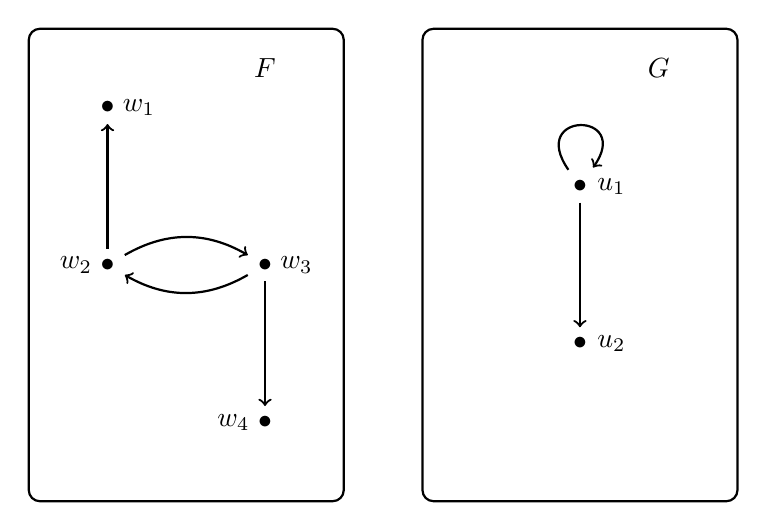
\begin{tikzpicture}[node distance=2cm, auto, thick]
    \node (w1) {$\bullet$};  %edge [in=55,out=125,loop] (); 
    \node (w2) [below of=w1] {$\bullet$}; 
    \node (w3) [right of=w2] {$\bullet$} ;
%    \node (fake) [right of=w3] {};
    \node (fake) at (4,-1) {};
    \draw[->] (w2) to node {} (w1); 
    \node (w4) [below of=w3] {$\bullet$} ; %edge [in=305,out=235,loop] ();
     \draw[->] (w3) to node {} (w4);
     \draw[->, bend left] (w3) to node {} (w2) ;
     \draw[->, bend left] (w2) to node {} (w3) ;
%    \draw[->, bend right] (w3) to node (w2); 
     \path node at ( 0.4,0) {$w_1$}; 
     \path node at ( -0.4,-2) {$w_2$}; 
     \path node at ( 2.4,-2) {$w_3$}; 
     \path node at ( 1.6,-4) {$w_4$};

     \draw [rounded corners] (-1,1) -- (-1,-5) -- (3,-5) -- (3,1) --  cycle;

     \path node at (2,0.5) {${F}$};

% \path node at ( 0,-1) [shape=circle,draw] {};
% \node [circle,draw] {a} edge [in=30,out=60,loop] ();

%     \node (u1) [right of=fake] {$\bullet$} edge [in=55,out=125,loop]
%     ();
     \node (u1) [right of=fake] {$\bullet$} edge [in=55,out=125,loop] ();
     \node (u2) [below of=u1] {$\bullet$} ;% edge [in=305,out=235,loop] ();
     \draw[->] (u1) to node {} (u2) ;
     \path node at (6.4,-1) {$u_1$};
     \path node at (6.4,-3) {$u_2$}  ;

     \draw [rounded corners] (4,-5) -- ++(4,0)  -- ++(0,6) -- ++(-4,0) --  cycle;

     \path node at (7,0.5) {${G}$};

  \end{tikzpicture}
\end{center}
\end{problem}

\begin{problem}  [15 points]
  Let the frames ${F}$ and ${G}$ be like in Problem
\olref{problem:frames}, and assume that the language only comprises
propositional variable $p_1, p_2, p_3$ for simplicity.
\begin{enumerate}
\item find valuations $U : \{p_1,p_2,p_3\} \to \Pow{W}$ and $V :
\{p_1,p_2,p_3\} \to \Pow{X}$ such that there is a $p$-morphism
between the models ${M} = ({W}, R, U)$ and ${N} = ({X}, S, V)$.
\item Are there valuations $U$ and $V$ such that the corresponding
  models are not $p$-morphic?
\end{enumerate}
\end{problem}


\begin{problem}  [15 points]
  Let $\pi$ be a $p$-morphism between models ${M} =
  ({W}, R, U)$ and ${N} = ({X}, S, V)$. Show that
  for any !!{formula} $!A$ and world $w \in {W}$, 
  \[
  \mSat{M}{!A}[w] \text{ if and only if }
  \mSat{N}{!A}[\pi(w)].
  \]
\end{problem}

\begin{problem}  [15 points]\ollabel{problem:AE}
  Show that for any model ${N}$ on ${G}$ there is a model ${M}$ on
  ${F}$ and a $p$-morphism $\pi$ from ${M}$ onto ${N}$.
\end{problem}

\begin{problem} [10 points]
  Show that the converse to Problem \olref{problem:AE} does not hold,
    i.e., that there is a model on ${F}$ that is not
    $p$-morphic to any model on ${G}$.
\end{problem}

\begin{problem} [10 points]\ollabel{problem:valid}
  Show that if !!a{formula} $!A$ is valid on $\mModel{F}$ then it is
  valid on $\mModel{G}$.\footnote{Warning. This requires showing that
    if $!A$ is true in any model on $\mModel{F}$ then it is true
    in any model on $\mModel{G}$. Use Problem \olref{problem:AE}.}
\end{problem}

\begin{problem} [10 points]
  Show that the converse of Problem \olref{problem:valid} does not hold,
  i.e., that there is !!a{formula} $!A$ that is valid on $\mModel{G}$ but
  not on $\mModel{F}$.\footnote{Hint. Consider !!a{formula} that says: `At any
    non-terminal world: if $!A$ is true and also true at any
    accessible terminal world, then $!A$ is necessary.'
%    $\lnot \Box\lfalse \lif \left[(!A \land \Box(\Box\lfalse \to
%      !A)) \lif \Box!A]$
}
\end{problem}



\begin{problem}  [15 points]
  The schema $T$, i.e., $\Box!A \lif !A$ is valid in a frame
  if and only if the frame is reflexive. Is there a schema that is
  valid in a frame if and only if the frame is \emph{irreflexive}?
\end{problem}







\section{Problem set 4: pebble games over Kripke frames}
\setcounter{problem}{0}



\begin{definition}[Two-pebble games on Kripke structures]
  Given two Kripke models ${M} = \tuple{W, R, U}$ and ${N} = \tuple{X,
    S, V}$ and worlds $u \in W$ and $v \in X$, the \emph{two-pebble
    game} $G({M}, u : {N}, v)$ between Abelard (``Abe the Spoiler'')
  and Elo\"ise (``Elly the Defender'') is defined as follows.

  Abelard and Elo\"ise share two pebbles, which at the beginning of
  the game are placed on the worlds $u$ and $v$.  A \emph{round} in
  the game begins with Abelard's sliding one of the pebbles along the
  accessibility relation ($R$ in ${M}$ or $S$ in ${N}$).  Elo\"ise
  likewise responds by sliding the other pebble along $S$ or $R$,
  respectively. In this way, two worlds $u'$ and $v'$ are identified
  such that $Ruu'$ and $Svv'$. If neither player wins the game at this
  round (as explained below), then both players advance and play a
  round of the game $G({M}, u' : {N}, v')$. Suppose the pebbles are on
  worlds $u \in W$ and $v\in X$; this configuration is assessed as a
  \emph{win} in the game $G({M}, u : {N}, v)$ for one or the other
  players based on whether the following conditions hold:
  \begin{enumerate}
  \item If there is an atomic sentence $p$ true at $u$ and false at
    $v$, or vice-versa, it's an automatic win for Abelard.
    \item If the worlds $u$ and $v$ are both terminal, it's an
      automatic win for Elo\"ise.
  \item If at any point Elo\"ise cannot slide her pebble to match
    Abelard's move, he wins.
  \item If the game goes on forever, that counts as a win for
    Elo\"ise. 
  \end{enumerate}
\end{definition}
 
 \begin{definition}
   A \emph{strategy} for either player in the game $G({M}, u :
   {N}, v)$ is just a function prescribing a response to each
   possible move of the other player. A \emph{winning strategy} is
   strategy that guarantees a win for the player following it.
 \end{definition}

\begin{problem}
  Show that if Abelard does \emph{not} have a winning strategy in the game
  $G({M}, u : {N}, v)$ then for any modal !!{formula}
  $!A$ we have $\mSat{M}{!A}[u]$ if and only if
  $\mSat{N}{!A}[v]$. 
\end{problem}


\end{document}

